\documentclass[9pt,twocolumn,a4paper]{article}
\usepackage{amssymb,amsmath,graphicx,soul,color,indentfirst}
\usepackage[affil-it]{authblk}



\newcommand*{\eg}{e.g. }
\newcommand*{\ie}{i.e. }



\begin{document}

\author{Aldosary, Buthainah\\
\texttt{aldosa@encs.concordia.ca}}
\affil{Concordia University\\
 Montreal, Canada}

\date{}
\title{Software Complexities: Do System and Change Complexity Relate?}




\maketitle
\section{Abstract}
\section{Introduction}

Traditional complexity measures are normalized on or require a whole file or system and were not designed to measure the complexity of code fragments. Therefor, the complexity of a change can be very different from the complexity of the files or system that contain a change (e.g a change to many simple files might be as complex as a change to one difficult file). Change complexity is related to, ``how hard is it to understand and review a change" vs system complexity, which measures for example, "how hard is it to understand and potentially modify the system". Traditional complexity measures do not really measure the complexity of the system but simply the size of the files that make up the system. As a result, they do not add any additional information beyond how large a file is. In contrast, all of the change complexity measures are based upon the notion that changes that are farther from each other or involve multiple entities are more complex than those closer together involving fewer entities. The goal of this paper is to evaluate the correlation between system complexity measures and change complexity measures of an evolving system. 
\newline

\textbf{We have the following research questions:}

\begin{enumerate}

\item Does the difference of traditional complexity measures before and after a change correlate with change complexity measures?

\item Does the weighted sum of change complexity measures up to a version correlated with the traditional complexity measures at that version? 

\item Do the traditional measures calculated on only the files that had changed at a certain commit correlate with the change complexity measures at the last 1000 changes?

\end{enumerate}

\section{Background and Motivation}

Traditional complexity metrics require the system as a whole and were not designed to measure the complexity of code fragments. McCabe’s metrics directly measures the number of linearly independent paths through a program's source code. Syntactic complexity metrics that are exclusively based on the structure of the program and the properties of the text (for example, redundancy of operators and operands, as Halstead’s metrics do), do not add any more information than lines of code do. [Isreal]. Furthermore, multiple studies have shown that these measures correlate very strongly with lines of code and may not provide additional information about the complexity of the system. [54,85,61].
As previously stated, measuring the complexity of a change differs from measuring an entire system. For example, a change to numerous simple functions across multiple files may be as difficult as changing the code contained within a single complex function. [Peter].
In this section, we provide a background on the various measures of system and change complexity.


\subsection{System (Traditional) Complexity Measures}
{\bf{\emph{Metrics Related to Lines of Code}}}
\newline
\begin{enumerate}

\item{\bf{Source Line of Code(SLOC): }} To define SLOC, we use the definition given by Conte [Conte 1986]: A line of code is any line of program text that is not a comment of blank line, regardless of the number of statements or fragments of statements on the line. This specifically includes all lines containing program headers, declarations, and executable and non-executable statements.

\item{\bf{Lines of Code (LOC): }} Lines of code refers to the total number of lines in each source code file including comments and blank lines


\item{\bf{BLANK: }}Blank is a count of the number of blank lines.

\item{\bf{COM.L: }}Number of lines that are exclusively comments (no code).

\item{\bf{COM.N: }} Number of comments in the file (a comment can be multiline).
\end{enumerate}


{\bf{\emph{Metrics Related to Complexity}}}
\newline

{\bf{McCabe's Cyclomatic Complexity}}\newline

McCabe’s Cyclomatic complexity is one of the earliest complexity measures developed by Thomas J. McCabe in 1976. It directly measures the number of linearly independent paths through a program's source code. Any program can be represented as a graph with the simplest element being a flat series of statements with no conditions, loops or branches. [Isreal] For a graph $G$ with $n$ vertices, $e$ edges and $p$ exit points, the complexity $v$ is defined as follows:

\begin{equation}
v(G)=e-n+2p
\end{equation}

It is worth mentioning that the minimum value for the cyclomatic complexity metric is 1, which corresponds to the flat series of statements with no bifurcations or loops. Every additional region in the flow graph would increase the Cyclomatic complexity by one unit.
\begin{enumerate}
\item{\bf{ (TOTCY)}}: Total McCabe's cyclomatic complexity (sum of all functions)
\item{\bf{MAXCY: }} Maximum McCabe’s cyclomatic complexity. (between all functions).

\item{\bf{MINCY: }} Minimum McCabe’s cyclomatic complexity.
\item{\bf{AVGCY: }} Average McCabe’s cyclomatic complexity.
\item{\bf{MEDCY: }} Median McCabe’s cyclomatic complexity.

{\bf{Halstead's Complexity Measures}}

Halstead’s complexity metrics rely on the idea that programs should be viewed as expressions of languages both programming and written. It relies on the premise that there are mathematically sound relationships among the number of variables, the complexity of the code and the type of programming language statements used.

\item{\bf{H.LEN: }}Halstead’s length.
\item{\bf{H.VOL: }}Halstead's volume.

\item{\bf{H.LEVEL: }}Halstead’s level.

\item{\bf{H MEN.D: }}Halstead’s number of mental discriminations.



\end{enumerate}

\subsection{Change Complexity Measures}

Since the goal of each measure is the same, to assess the complexity of a change, we expect some of our measures to be highly correlated. In the interest of parsimony, we will select the simplest set of measures that adequately captures change complexity.

\begin{enumerate}

\item{\bf{Files and diffs (Mods)}}: We count the number of files contained in a commit. The more files that change, the larger the affect proportion of the system. Commits with a large number of files will likely be difficult to understand.

\item{\bf{Change blocks (Hunks)}}: We measure the number of contiguous change blocks, or hunks, and the distance between these blocks in a modified file and sum them across the entire review. Contiguous changes are likely easier to review than changes that are further apart and that are potentially in multiple functions within a file.

\item{\bf{Indentation: [Hindle2008ICPC]}} creates a complexity measure that can be used to measure the complexity of the entire system or of a change by examining the level of indentation on source lines. We calculate their measure for reviews. They found that the strongest predictors of complexity were the sum and standard deviation of the indentation of source lines.

\end{enumerate}


%TODO weighted number of people who changed a file?

\section{Methodology and Data}

A quantitative research methodology was used for this empirical study where the objective was to develop models pertaining to our research questions. The choice of this method is key as it provides a connection between the empirical observation and mathematical expressions of the quantitative relationships. 
The data used for this study was provided by Dr. Peter Rigby, namely from the Apache HTTP Server Project written in C. All measures were calculated at a particular version (commit) and the data was retrieved from June 18, 1999 – March 3, 2011; that is during a 12 year time period. SQL scripts were written to extract data of system and change complexity measure that answer each of the research questions using PostgreSQL 9.3. The resulting data was then imported into RStudio for further analysis. Finally, Spearman’s rank correlation coefficient matrix was deduced for each measure. 


In figure 1 we illustrate a hypothetical system which undergoes numerous changes. The vertical lines represent each version. During each version's development, the change complexity measures are assessed. In between versions, traditional complexity measures are computed. These are denoted by CCM and TCM respectively.

\begin{figure}[h!]
  \centering
  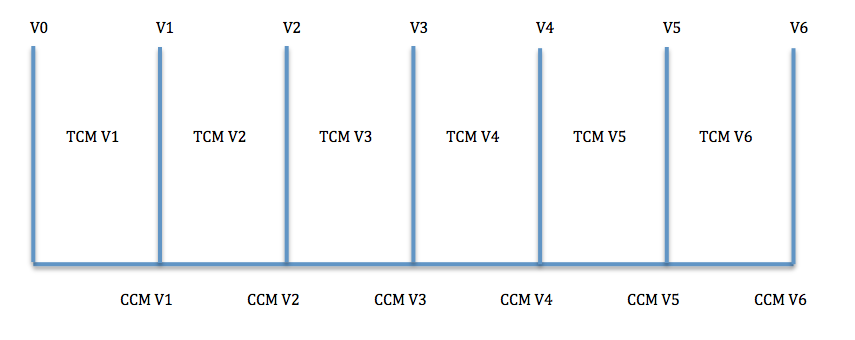
\includegraphics[width=0.5\textwidth]{change_complexity_figure}
   \caption{"Change Complexity vs. Traditional Complexity"}
\end{figure}

\begin{equation}
{{CCM_{v(i)}} = {TCM_{v(i+1)}}-{TCM_{v(i)}}}
\end{equation}

\begin{equation}
{{TCM_{v(i+1)}} = \sum\limits_{i=0}^iCCM_{v(i)}}
\end{equation}
 
\begin{equation}
{{{TCM_{v(i)}} = CCM_{v(i)}}   _{n=1000}}
\end{equation}

\section{Results and Discussion}

It has been previously shown that Halstead’s length, volume, level and mental discriminations all correlate highly with each other [Israel], so it is safe to select hlen only of these metrics. Maxcy and sloc have also shown to correlate highly with each other so Maxcy has been chosen. Total cyclomatic complexity has been also added as it provides the complexity measure for the sum of all functions. Finally, loc has been included as it’s a measure of all text lines in the code. For measures pertaining to change complexity, we have chosen the simplest ones that adequately capture change complexity. 
\newline

{\bf{\emph Q1) Does the difference of traditional complexity measures before and after a change correlate with change complexity measures?}}
\newline

We measure the difference between traditional complexity measures before and after a change and relate that with the change complexity measure at that particular change. By examining the result, we can see that measures that are related to change complexity correlate very poorly with those of system complexity (\textless 0.3).
\newline

\begin{table}[ht]

\centering
\resizebox{8cm}{!}{
\begin{tabular}{r||rrrrrrr}
  \hline
 & mods & hunk\_dist & indent\_sum & loc & hlen & maxcy & totcy \\ 
  \hline
mods & 1.00 & 0.65 & 0.85 & 0.30 & 0.26 & 0.23 & 0.26 \\ 
  hunk\_dist & 0.65 & 1.00 & 0.63 & 0.18 & 0.16 & 0.11 & 0.14 \\ 
  indent\_sum & 0.85 & 0.63 & 1.00 & 0.28 & 0.24 & 0.22 & 0.24 \\ 
  loc & 0.30 & 0.18 & 0.28 & 1.00 & 0.89 & 0.54 & 0.73 \\ 
  hlen & 0.26 & 0.16 & 0.24 & 0.89 & 1.00 & 0.51 & 0.70 \\ 
  maxcy & 0.23 & 0.11 & 0.22 & 0.54 & 0.51 & 1.00 & 0.64 \\ 
  totcy & 0.26 & 0.14 & 0.24 & 0.73 & 0.70 & 0.64 & 1.00 \\ 
   \hline
\end{tabular}}
\caption {\small Correlation Matrix of Research Question 1.}
\label{tab:title} 
\end{table}

{\bf{\emph Q2)Does the weighted sum of change complexity measures up to a version correlated with the traditional complexity measures at that version? }}
\newline

We measured the last 1000 commits’ weighted sum of change complexity measures up to a single version and compared it with the traditional complexity measures of that version. By looking at the results in the following table, we can see that change complexity measures correlated negatively with traditional complexity measures.
\newline

\begin{table}[ht]
\centering
\resizebox{8cm}{!}{
\begin{tabular}{r||rrrrrrr}
  \hline
 & mods & hunk\_dist & indent\_sum & loc & hlen & maxcy & totcy \\ 
  \hline
mods & 1.00 & 0.25 & 0.96 & -0.23 & -0.21 & -0.38 & -0.36 \\ 
  hunk\_dist & 0.25 & 1.00 & 0.31 & -0.21 & -0.22 & -0.19 & -0.20 \\ 
  indent\_sum & 0.96 & 0.31 & 1.00 & -0.18 & -0.16 & -0.32 & -0.30 \\ 
  loc & -0.23 & -0.21 & -0.18 & 1.00 & 1.00 & 0.95 & 0.96 \\ 
  hlen & -0.21 & -0.22 & -0.16 & 1.00 & 1.00 & 0.94 & 0.95 \\ 
  maxcy & -0.38 & -0.19 & -0.32 & 0.95 & 0.94 & 1.00 & 1.00 \\ 
  totcy & -0.36 & -0.20 & -0.30 & 0.96 & 0.95 & 1.00 & 1.00 \\ 
   \hline
\end{tabular}}
\caption {\small Correlation Matrix of Research Question 2.}
\label{tab:title} 
\end{table}


{\bf{\emph Q3)Do the traditional measures calculated on only the files that had changed at a certain commit correlate with the change complexity measures at the last 1000 changes?}}
\newline

To answer the third research question, first we identified the files that have undergone changes in a version and extracted the traditional measures for them. Then, we measured the change complexity measures for the last 1000 changes and compared these two measures.  Table 3 (???) shows the correlation matrix which shows that there is a very poor correlation between the change complexity measures and traditional complexity measures (\textless 0.3).

\begin{table}[ht]

\centering
\resizebox{8cm}{!}{
\begin{tabular}{r||rrrrrrr}
  \hline
 & mods & hunk\_dist & indent\_sum & loc & hlen & maxcy & totcy \\ 
  \hline
mods & 1.00 & 0.66 & 0.86 & 0.23 & 0.23 & 0.21 & 0.23 \\ 
  hunk\_dist & 0.66 & 1.00 & 0.63 & 0.27 & 0.26 & 0.22 & 0.28 \\ 
  indent\_sum & 0.86 & 0.63 & 1.00 & 0.26 & 0.26 & 0.28 & 0.27 \\ 
  loc & 0.23 & 0.27 & 0.26 & 1.00 & 0.99 & 0.82 & 0.96 \\ 
  hlen & 0.23 & 0.26 & 0.26 & 0.99 & 1.00 & 0.85 & 0.96 \\ 
  maxcy & 0.21 & 0.22 & 0.28 & 0.82 & 0.85 & 1.00 & 0.84 \\ 
  totcy & 0.23 & 0.28 & 0.27 & 0.96 & 0.96 & 0.84 & 1.00 \\ 
   \hline
\end{tabular}}
\caption {\small Correlation Matrix of Research Question 3.}
\label{tab:title} 
\end{table}




\section{Threats to validity}

\section{Conclusion}

Future work: Does McCabe predict anything? Do the change complexity measures do a better job of prediction?

\end{document}
